\section{Interfaccia utente}

\subsection{Homepage}
La homepage è la prima schermata che l'utente visualizza all'apertura
dell'applicazione. L'elemento principale è un menu a tendina, situato al centro
della pagina: esso contiene una lista di dataset\textsubscript{g}, ognuno dei quali rappresenta
un argomento di studio diverso.
\begin{figure}[ht!]
    \centering
    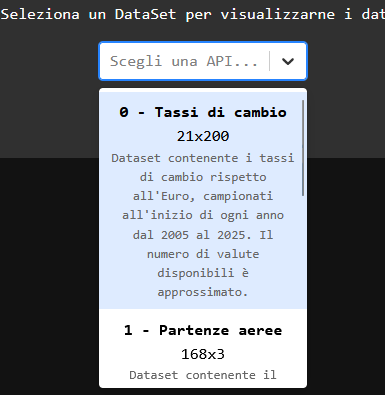
\includegraphics[scale=0.5]{template/images/home/options.png}
    \caption{Menu a tendina}
\end{figure}

Scegliendo un'opzione dal menu, l'utente può visualizzare le informazioni
relative a quel dataset\textsubscript{g}:
\begin{itemize}
    \item Nome del dataset\textsubscript{g};
    \item Dimensioni del dataset\textsubscript{g} (numero di righe e di colonne);
    \item Breve descrizione del dataset\textsubscript{g}.
\end{itemize}
\begin{figure}[ht!]
    \centering
    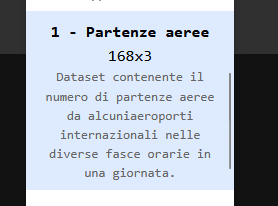
\includegraphics[scale=0.5]{template/images/home/dataset.png}
    \caption{Informazioni relative a un dataset\textsubscript{g}}
\end{figure}
Inoltre, premendo il pulsante "Avanti", l'utente può avviare il caricamento del
dataset\textsubscript{g} selezionato. Al termine del caricamento, l'utente viene reindirizzato
all'ambiente 3D associato al dataset\textsubscript{g}.
\begin{figure}[ht!]
    \centering
    
\includegraphics[scale=0.6]{template/images/home/btn.png}
    \caption{Pulsante "Avanti"}
\end{figure}

\subsection{Ambiente 3D}
L'ambiente 3D è la schermata principale in cui l'utente può visualizzare i dati
e interagire con essi. Il nome del dataset\textsubscript{g} è situato in alto al centro dell'ambiente.
La pagina comprende i seguenti elementi:
\begin{itemize}
    \item \textbf{Grafico 3D\textsubscript{g}:} rappresenta il dataset\textsubscript{g} selezionato e consente di
          interagire con esso;
    \item \textbf{Form delle opzioni:} può essere reso visibile premendo
          il pulsante situato in alto a destra. Consente di filtrare i dati in
          base a criteri specifici e modificare le opzioni di visualizzazione;
    \item \textbf{Tabella dei dati:} può essere resa visibile premendo il
          pulsante in basso a sinistra. Mostra il dataset\textsubscript{g} in forma tabellare e
          consente di interagire con esso.
\end{itemize}
\begin{figure}[ht!]
    \centering
    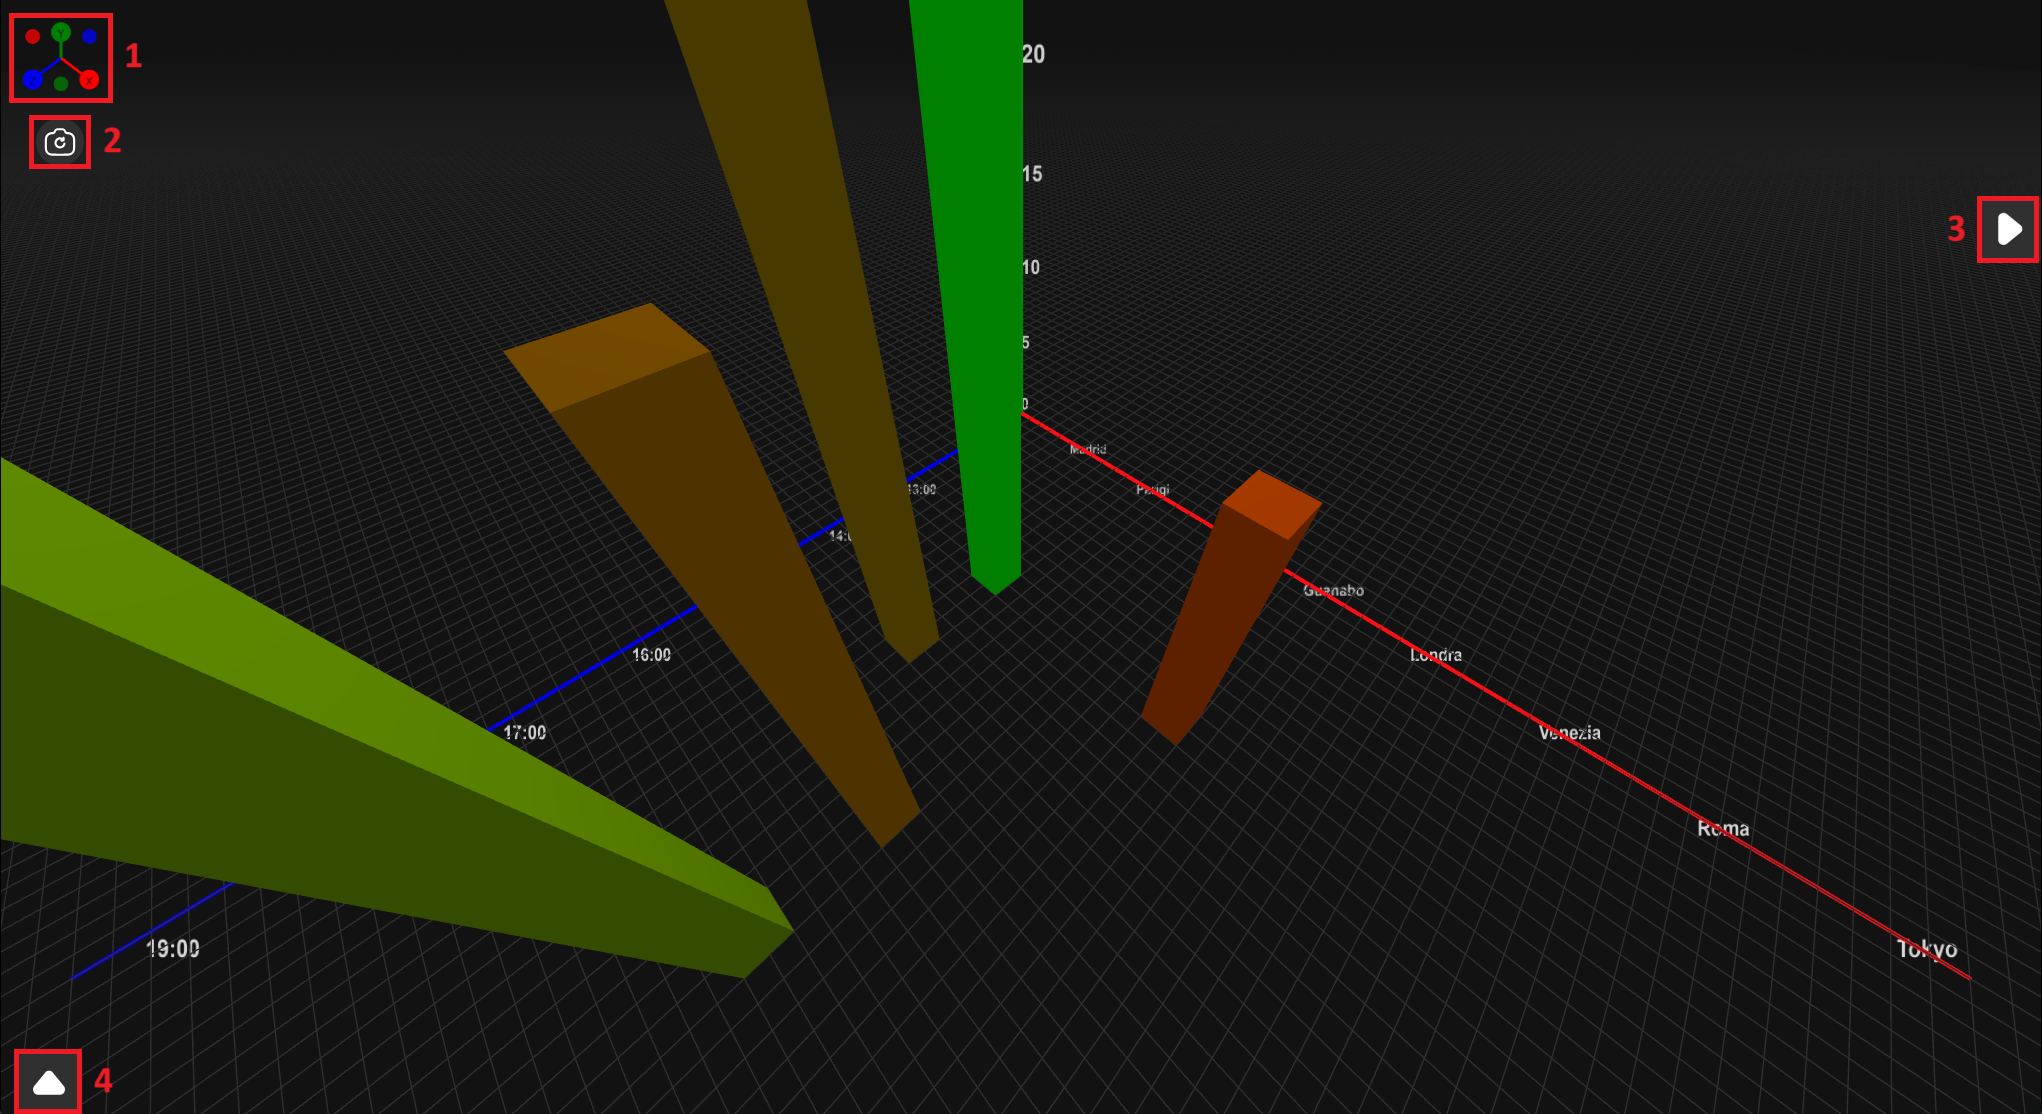
\includegraphics[scale=0.29]{template/images/envpage.png}
    \caption{Ambiente 3D con elementi interattivi numerati}
    \begin{flushleft}
        \hspace{5.45cm}(1) Gizmo\textsubscript{g}\\
        \hspace{5.45cm}(2) Pulsante di reset della visualizzazione\\
        \hspace{5.45cm}(3) Pulsante per il form delle opzioni\\
        \hspace{5.45cm}(4) Pulsante per la tabella
    \end{flushleft}
\end{figure}
\subsubsection{Grafico 3D}
Il grafico 3D\textsubscript{g} è l'elemento centrale dell'ambiente 3D e rappresenta il dataset\textsubscript{g}
selezionato. Ogni barra\textsubscript{g} del grafico rappresenta un valore specifico del
dataset\textsubscript{g}, mentre l'altezza della barra\textsubscript{g} indica il valore stesso. Le barre\textsubscript{g} sono
colorate in base al loro valore, con una scala di colori che va dal rosso
(valori bassi) al verde (valori alti).

\subsubsection{Form delle opzioni}
Il form delle opzioni consente di filtrare i dati in base a criteri specifici e
modificare le opzioni di visualizzazione. Può essere reso visibile oppure
nascosto premendo il pulsante situato in alto a destra nell'ambiente 3D.
Procedendo dall'alto verso il basso, il form è composto da:
\begin{itemize}
    \item Pulsante per filtrare i valori superiori o inferiori (a seconda dell'opzione
          selezionata) al valore medio\textsubscript{g} del dataset\textsubscript{g};
    \item Campo di input per inserire un numero intero positivo;
    \item Pulsante per filtrare i primi N valori più alti o più bassi (a seconda
          dell'opzione selezionata) del dataset\textsubscript{g}, dove N è il numero inserito nel campo di
          input;
    \item Pulsanti di opzione per scegliere se filtrare i valori più alti o più bassi,
          relativamente a qualunque filtraggio;
    \item Pulsante per rimuovere il filtro applicato;
    \item Pulsanti di opzione per scegliere se visualizzare o meno il piano parallelo al
          piano XZ (base del grafico), che mostra il valore medio\textsubscript{g} del dataset\textsubscript{g}.
\end{itemize}
\begin{figure}[ht!]
    \centering
    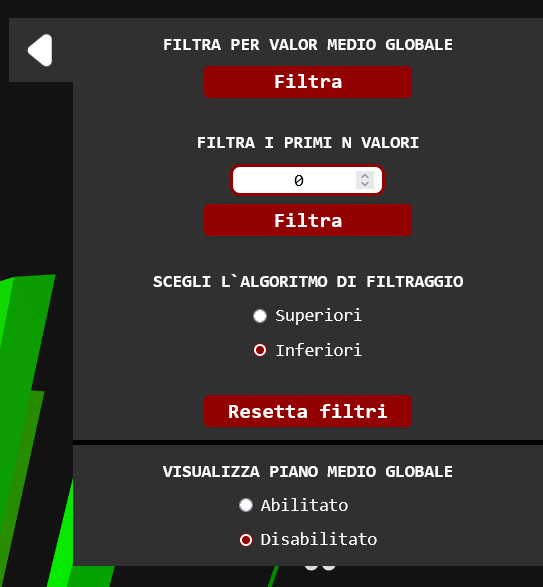
\includegraphics[scale=0.6]{template/images/env/options.png}
    \caption{Form delle opzioni}
\end{figure}

\subsubsection{Tabella dei dati}
La tabella dei dati mostra il dataset\textsubscript{g} in forma tabellare e consente di
interagire con esso. Può essere resa visibile oppure nascosta premendo il
pulsante situato in basso a sinistra nell'ambiente 3D.\\ La prima colonna
contiene le intestazioni delle righe, che rappresentano le etichette dell'asse
X del grafico. La prima riga contiene le intestazioni delle colonne, che
rappresentano le etichette dell'asse Z del grafico. Le celle della tabella
contengono i valori del dataset\textsubscript{g} e possono assumere colori diversi a seconda che
la corrispondente barra\textsubscript{g} del grafico sia visibile o meno.
\begin{figure}[ht!]
    \centering
    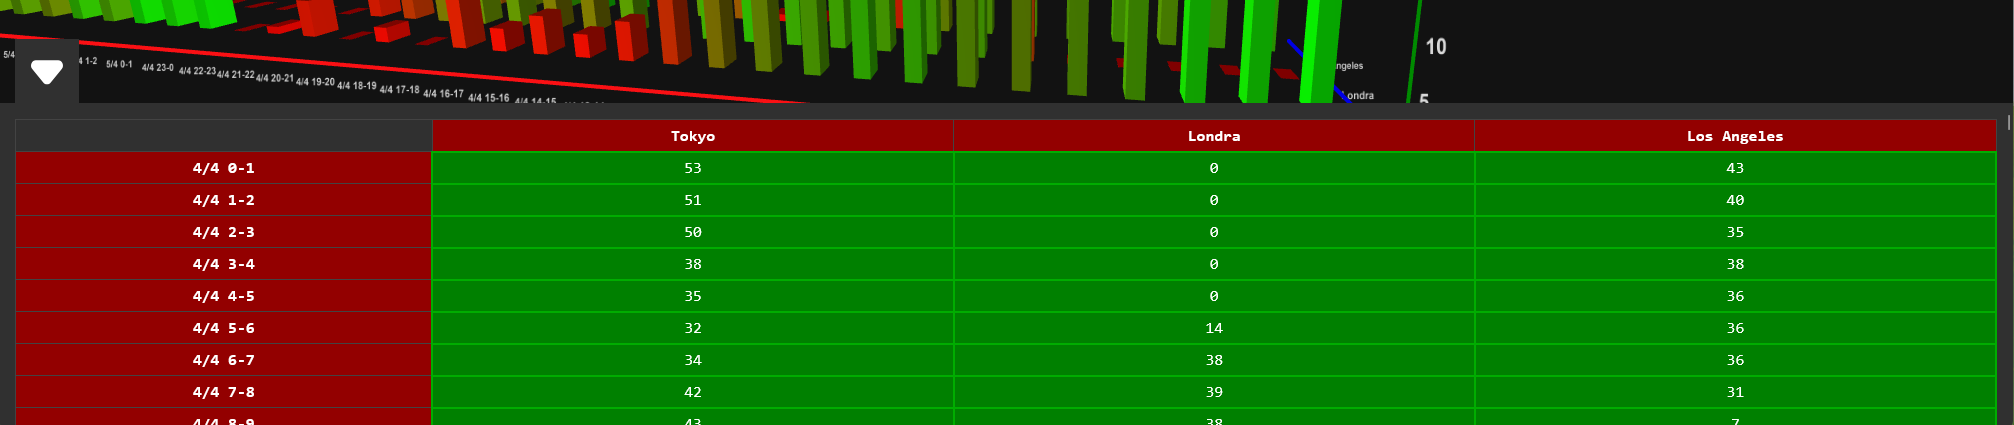
\includegraphics[scale=0.3]{template/images/env/table.png}
    \caption{Tabella dei dati}
\end{figure}